\documentclass{article}
\usepackage[en]{ukon-infie}
\usepackage[utf8]{inputenc}
\usepackage{algorithm2e}
\usepackage{amsmath}
\usepackage{graphicx}
% kann de oder en sein
% kann bubble break, topexercise sein

\Names{Jonas Probst, Simon Giebenhain}
\Lecture[AnaVis]{Analyse und Visualisierung von Informationen}
\Term{WS 2017/18}

\begin{document}
    \begin{ukon-infie}[10.01.18]{8}

        \begin{exercise}[p=3]{Theoretical Questions}  
        \question{}
        {
        	Find patterns in Datasets that frequently occur together.
        }
    	\question{}
    	{
    		Classification tries to classify datapoints into known classes, AR Mining tries to find datapoints that frequntly occur together.
    	}
    	\question{}
    	{
    		Clustering tries to find similar datapoints, AR mining doesn't care about similarity only about datapoints occuring together.
    	}
    	\question{}
    	{
			$buys$(X, "milk") $\Rightarrow$ $buys$(X, "cereal") \\
			A rule stating what is frequently bought together, given with a certain support and frequency (see next question).   	
    	}
    	\question{}
    	{
			$buys$(X, "milk") $\Rightarrow$ $buys$(X, "cereal"), $support=5\%$\\ $5\%$ of transactions showed milk and cereal bought together.
    	}
    	\question{}
    	{
			$buys$(X, "milk") $\Rightarrow$ $buys$(X, "cereal"), $confidence=50\%$\\
			If a customer buys milk there is a $50\%$ chance he buys cereal as well.   	
    	}
    	

		\end{exercise}
		
		\begin{exercise}[p=2+2+1+1]{FP-Tree Algorithm}
		\question{}{

\begin{tabular}{|l|l|l|l|}
\hline
ID & Items         & \begin{tabular}[c]{@{}l@{}}Ordered list of \\textbackslash\\ 1-itemsets\end{tabular} & \begin{tabular}[c]{@{}l@{}}ordered \\textbackslash\\ frequent items\end{tabular} \\ \hline
1  & \{M,H,C,A,G\} & M:8                                                                                  & \{M,G,A,C\}                                                                      \\ \hline
2  & \{M,H,C,G\}   & G:6                                                                                  & \{M,G,C\}                                                                        \\ \hline
3  & \{M,A,G\}     & A:5                                                                                  & \{M,G,A\}                                                                        \\ \hline
4  & \{M,C,A,F\}   & C,F:4                                                                                & \{M,A,C,F\}                                                                     \\ \hline
5  & \{M,A,G,F\}   & H:3                                                                                  & \{M,G,A,F\}                                                                      \\ \hline
6  & \{M,A,G,F\}   & E:1                                                                                  & \{M,G,A,F\}                                                                      \\ \hline
7  & \{M,C,E,F\}   &                                                                                      & \{M,C,F\}                                                                        \\ \hline
8  & \{M,H,G\}     &                                                                                      & \{M,G\}                                                                          \\ \hline
\end{tabular}
}\\
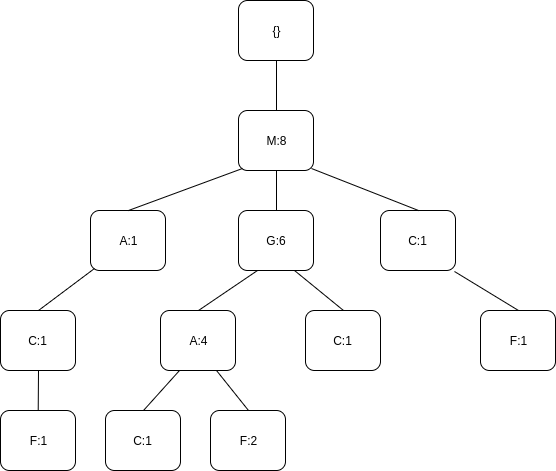
\includegraphics[scale=0.5]{FPtree.png}

		\question{}
		{
		\begin{tabular}{|l|l|}
\hline
Item & Conditional Pattern Base \\ \hline
G:6  & M:6                      \\ \hline
A:5  & MG:4, M:1                \\ \hline
C:4  & MA:1, MGA:1, MG:1, M:1   \\ \hline
F:4  & MGA:2, MAC:1, MC:1       \\ \hline
\end{tabular}
		}

		\end{exercise}
		
		
\end{ukon-infie}
\end{document}
